\section{Testing Methodologies}\label{sec:methodology}

This section describes our approach for classifying the outcomes of test cases, and for voting on these outcomes in order to expose anomalous compiler behavior.


\subsection{Classifying Test-case Outcomes}

\begin{figure}
  \centering %
  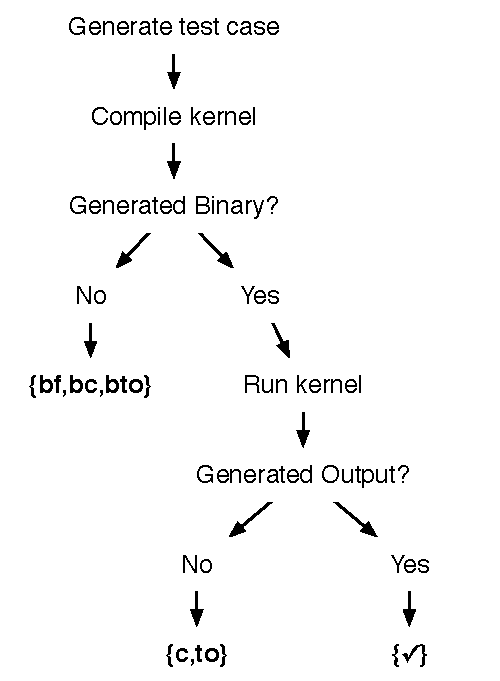
\includegraphics[width=.62\columnwidth]{img/test_process}%
  \caption{%
    Test-case execution, and possible outcomes. Each test-case execution produces one of six possible outcomes: \{bf,bc,bto,c,to,\cmark\}.%
  }%
\label{fig:test-process} %
\end{figure}

% We classify the result of executing a test-case into one of six classifications: build failure (\textbf{bf}), build crash (\textbf{bc}), runtime crash (\textbf{c}), or pass (\textbf{\cmark}). A \textbf{bf} occurs when compilation of a kernel fails, usually accompanied by an error message. A \textbf{bc} outcome occurs when the compiler crashes. A \textbf{c} outcome occurs when the program crashes during execution. The \textbf{bto} and \textbf{to} outcomes occur when the program compilation or execution time out, respectively.

A \emph{build failure} (\textbf{bf}) occurs when online compilation of the OpenCL kernel fails, usually accompanied by an error diagnostic. A \emph{build crash} (\textbf{bc}) or \emph{build timeout} (\textbf{bto}) outcome occurs if the compiler crashes or fails to produce a binary within 60 seconds, respectively. For compile-only test-cases, a \emph{pass} (\textbf{\cmark}) is achieved if the compiler produces a binary. For test-cases in which the kernel is executed, kernel execution leads to one of three potential outcomes: \emph{runtime crash} (\textbf{c}) if the program crashes, \emph{timeout} (\textbf{to}) if the kernel fails to terminate within 60 seconds, or \emph{pass} (\textbf{\cmark}) if the kernel terminates gracefully and computes an output. 
%
%\begin{enumerate}
%	\item \emph{Build failure} (\textbf{bf}) Online compilation of the OpenCL kernel fails, usually accompanied by an error diagnostic.
%	\item \emph{Build crash} (\textbf{bc}) The compiler crashes during online compilation of the OpenCL kernel.
%	\item \emph{Build timeout} (\textbf{bto}) Online compilation of the OpenCL kernel exceeds the timeout of 60 seconds.
%	\item \emph{Runtime crash} (\textbf{c}) Compilation of the OpenCL kernel succeeds gracefully, but the program crashes during kernel execution.
%	\item \emph{Runtime timeout} (\textbf{to}) Compilation of the OpenCL kernel succeeds gracefully, but program execution exceeds the timeout of 60 second.
%	\item \textbf{\cmark} \emph{Completion} The program terminates gracefully and produces an output.
%\end{enumerate}

When evaluating the outcomes of test-cases, \textbf{\{bc,bto\}} outcomes are of immediate interest, indicative of erroneous compiler behavior. For all other outcomes, \emph{differential tests} are required to expose anomalous behavior.


\subsection{Voting Heuristics for Differential Testing}

As in previous work, we do not guarantee that generated programs time out, finding that XX\% of programs do not.

Prior works have require random programs be free from undefined and unspecified behaviour~\cite{Yang2011c,Le2013a,Le2015}. Recently, work in Skeletal Program Enumeration has relied on handchecking of C programs and tools such as CompCert and UBsan~\cite{Zhang2017a}. Our approach is closer to the latter, except that we do not even guarantee that generated programs are well-formed. Instead, we rely extensively on voting across configurations to reveal anomalous outputs.

Voting is used to expose anomalous outcomes from configurations. In prior work, voting has been used to determine wrong-code bugs. In~\cite{Lidbury2015a}, a configuration is determined to have produced a wrong code result for a kernel if there is a majority output of at least 3 among the \{\cmark\} results for the kernel, and the configuration yields a \{\cmark\} result that disagrees with the majority. We extend this approach to describe not only anomalous code bugs, but also anomalous build failures, crashes, and timeouts.

A majority exists if, for $n$ configurations, at least $\ceil{2n/3}$ configurations produce non-\textbf{bc} results with the same outcome. For \cmark majority outcomes, the output of the program is used.

Only 2.3\% of CLSmith programs with anomalous outputs are insensitive to optimization level.

%
\begin{enumerate}
	\item \textbf{w} \emph{Wrong code} Program terminates gracefully, but computes a result which differs from the majority output. For a DeepSmith result to be classified with \emph{wrong-code}, we require first that the program passes verification using GPUVerify~\cite{Betts2012}, and that a reference run with Oclgrind~\cite{Price2015} produces no warnings. \cc{Vote on compiler warnings, and optimization sensitivity. This means we way miss bugs which optimization level insensitive, though our experiences testing with CLSmith revelead only discovered 2 such cases}.
	\item \textbf{bf} \emph{Build failure} Online compilation of OpenCL program fails, whereas the majority of configurations produce a binary. \cc{TODO: voting to exclude programs which rely on OpenCL 2.0 / compiler specific features}
	\item \textbf{c} \emph{Runtime crash} One or more OpenCL API calls return an error status during the program execution, or the program crashes.
	\item \textbf{to} \emph{Runtime timeout} Program execution exceeds the timeout of 60 second, whereas the majority of configurations produce an output.
\end{enumerate}


\subsection{Discussions}

\paragraph{Undefined Behaviors} OpenCL doesn't have CompCert and UBSan. GPUverify and Oclgrind can catch some errors, so as we have shown in Section~\ref{sec:motivation}, no tool is perfect. Compiler errors are useful. There is much work to be done. We demand that the behavior of test-cases is \emph{portable} and \emph{reproducible}. In some respects this simplifies the execution process.


\paragraph{Floating Points} The OpenCL 1.2 specification permits acceptable error bounds (ULP) for floating point operations and builtin functions. Some operations like addition, subtraction, and multiplication are precise; divide permits a small error, and builtins vary widely. Thus two implementation may give different answers that both fit within the allowed ranges (and because errors propagate through operations it's hard to even describe the ULP on the final output). \texttt{half\_} functions permit large error bounds. \texttt{native\_} functions have ``implementation defined'' error bounds. TODO: Denormal numbers may optionally be pushed to zero.

\cc{If we difftest across floats:}
CSmith, and by extension, CLSmith, do not support floating point operations. In our observations with testing using CLSmith (described in Section~\ref{sec:vs_clsmith}), we observed that in cases of wrong-code bugs, the computed values are usually entirely incorrect, not only marginally different. We hypothesized that by allowing relaxed comparisons between floating point values, we could still differential test. We permit a margin of deviation for floating point comparisons. This means that if a compiler were to emit wrong code which changes the computed value only subtly, we may miss it; though we have no reason to suggest that such a case is any more likely than a wrong code bug leading the compiler to produce exactly the same output, which neither we or any prior work have noted.

\cc{If we ignore floats:}
Given that not all vendors provide bounds for floating point imprecision, we excluded kernels containing floating points from the wrong-code check. Given knowledge about hardware imprecision, it would be possible to compute threshold for floating point difftests.
% Section 7.4 of OpenCL 1.2 spec.
